\documentclass[11pt]{standalone}
\usepackage[utf8]{inputenc}
\usepackage{tikz}
\usetikzlibrary{calc,positioning,shapes.geometric,fit,arrows}
\usepackage{tgheros}

\begin{document}
  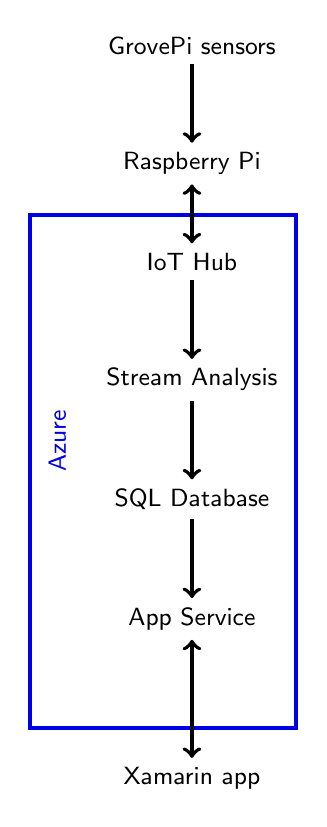
\begin{tikzpicture}[
  	font=\sffamily\small,
	linie/.style={
	draw=black,solid,line width=0.5mm,
	}
	]

\node (sensoren) {GrovePi sensors};
\node[below=of sensoren] (raspi) {Raspberry Pi};
\node[below=-0.5cm of raspi] (empty) {};
\node[below=of empty] (iothub) {IoT Hub};
\node[below=of iothub] (stream) {Stream Analysis};
\node[below=of stream] (sqldb) {SQL Database};
\node[below=of sqldb] (appservice) {App Service};

\node[anchor=south west,rotate=90,left=0.5cm of stream.south west, color=blue!90!black] (azuretext) {Azure};
\node[below=of raspi, draw=blue!90!black, line width=0.5mm, fit={(azuretext) (empty) (iothub) (stream) (sqldb) (appservice)}] (azure) {};

\node[below=1.5cm of appservice] (app) {Xamarin app};

\draw [->, linie] (sensoren) to (raspi);
\draw [<->, linie] (raspi) to (iothub);
\draw [->, linie] (iothub) to (stream);
\draw [->, linie] (stream) to (sqldb);
\draw [->, linie] (sqldb) to (appservice);
\draw [<->, linie] (appservice) to (app);

  \end{tikzpicture}
\end{document}